%%%%%%%%%%%%%%%%%%%%%%%%%%%%%%%%%%%%%%%%%%%%%%%%%%%%%%%%%%%%%%%%%%%%%%%%%%%%%%%
%                         File: osa-revtex4-1.tex                             %
%                        Date: April 15, 2013                                 %
%                                                                             %
%                              BETA VERSION!                                  %
%                   JOSA A, JOSA B, Applied Optics, Optics Letters            %
%                                                                             %
%            This file requires the substyle file osajnl4-1.rtx,              %
%                   running under REVTeX 4.1 and LaTeX 2e                     %
%                                                                             %
%                   USE THE FOLLOWING REVTeX 4-1 OPTIONS:                     %
% \documentclass[osajnl,twocolumn,showpacs,superscriptaddress,10pt]{revtex4-1}%
%                    %% Use 11pt for Applied Optics                           %
%                                                                             %
%               (c) 2013 The Optical Society of America                       %
%                                                                             %
%%%%%%%%%%%%%%%%%%%%%%%%%%%%%%%%%%%%%%%%%%%%%%%%%%%%%%%%%%%%%%%%%%%%%%%%%%%%%%%

%\documentclass[osajnl,twocolumn,showpacs,superscriptaddress,10pt]{revtex4-1} %% use 11pt for Applied Optics
\documentclass[osajnl,preprint,showpacs,superscriptaddress,12pt]{revtex4-1} %% use 12pt for preprint option
\usepackage{amsmath,amssymb,graphicx}
\usepackage{multirow}
\usepackage{setspace}
\usepackage{longtable}

\newcommand{\procspie}{{Proc. ~SPIE}}
\begin{document}

\title{Characterization of gaps in directly bonded Si compound optics}

\author{Michael Gully-Santiago}\email{gully@astro.as.utexas.edu}
\author{Daniel T. Jaffe}
\affiliation{Department of Astronomy, The University of Texas at Austin, Austin, TX, 78712, USA}

\author{Victor White}
\affiliation{NASA Jet Propulsion Laboratory, Pasadena, CA}


\begin{abstract}
Si direct bonding offers flexibility in the design and development of large Si optics.  The bonding process presents challenges in meeting the performance demands and physical robustness, in particular for cryogenic and space applications.  Air cavities in between the Si interface will have large Fresnel reflections which will interfere as a low-Finesse Fabry-P\`erot etalon.  Even small 35 nm gaps reduce transmission through a direct bonded Si compound optic by 5\% at $\lambda = $ 1.15 $\mu$m at normal incidence.  Stock near infrared spectrophotometers like the Cary5000 from Agilent offer 0.2\% photometric precision.  We can detect measure gaps as small as 8 nm by measuring transmission as a function of wavelength.  Our approach involves modeling multiple incoherent reflections within the substrate interfaces with a wave transfer matrix, modified for intensities rather than complex amplitudes.  The detection and morphology of minuscule gaps provides valuable feedback in the design of Si direct bonding strategies.
\end{abstract}

\ocis{(030.1670) Coherent optical effects; (050.2230) Fabry-Perot; (120.2230)   Fabry-Perot; (120.2830) Height measurements; (120.4610) Optical fabrication; (120.7000) Transmission; (120.7000)   Transmission; (220.4840) Testing; (230.4170) Multilayers; (240.1485) Buried interfaces;  (300.6340) Spectroscopy, infrared; (310.6628)  Subwavelength structures, nanostructures}

\maketitle %% required

\section{Introduction}


Direct optical bonding of silicon allows manufacturers to combine parts with no Fresnel loss at the interface.  The high refractive index of Si makes this advantage particularly useful.  Traditional figures of merit for the optical audits of bonds, however, are either insensitive to gaps that are small yet have a significant impact on throughput and phase coherence, or do not provide quantitative information about the extent of the gaps along the direction of propagation.

Issues with the quality of the bonds become particular acute when the optics are used in double-pass and/or when the incidence angle at the bonds is far from the normal.

The University of Texas diffractive optics group produces diffraction gratings on silicon using microlithographic techniques \cite{1998SPIE.3354..201J,2010SPIE.7739E.146W}.  These gratings are used either in transmission (i.e. as grisms \cite{2008SPIE.7014E..77D, 2010SPIE.7739E.123G}), or in reflection (i.e. as immersion gratings, \cite{2007ApOpt..46.3400M, 2010SPIE.7739E.146W,2012SPIE.8450E..2SG}.  These gratings operate throughout the infrared, from 1.2 to 38 $\mu$m, and find application in ground-based (IGRINS \cite{2010SPIE.7735E..54Y, 2012SPIE.8450E..2SG}), airborne (SOFIA FORCAST \cite{2008SPIE.7014E..77D}), and space (JWST NIRCAM \cite{2005SPIE.5904...21B,2010SPIE.7739E.123G}) applications.  To date, our group has produced the gratings on large (up to 100 mm diameter and 30 mm thick) monolithic pieces of monocrystalline silicon and we shape the substrates by sawing, grinding, and polishing to form the final devices \cite{2010SPIE.7739E.146W}.  The next generation of astronomy and earth science spectrographs, however, will need optical devices larger and more precise than what can be made with existing technology.  The proposed Giant Magellan Telescope \cite{2012SPIE.8444E..1HJ} Near Infrared Spectrograph \cite{2006SPIE.6269E.143J,2010SPIE.7735E..87L} (GMTNIRS) will need immersion gratings with thicknesses up to 60 mm and lengths up to 200 mm.  Substrates of the required size cannot fit into conventional processing equipment like reactive ion etchers and electron-beam lithography tools.  Large, thick Si substrates are also prohibitively expensive to experiment on.  Silicon direct bonding \cite{1986JAP....60.2987S,2012SPIE.8450E..2TV} offers advantages by reducing the thickness and mass needed for the development of a thin (0.5$-$10 mm) Silicon diffractive optic that can later be bonded to a fine polished Si prism substrate.  Other groups producing SI diffractive optics are also experimenting with this approach (see \cite{2012SPIE.8450E..2TV} and \url{www.lumella.com}).


While it is possible that proper precautions to eliminate all micron-sized particles from both SI surfaces prior to bonding, the power-law nature of the particle size distribution in clean-room environments (\cite{Cooper_1986}) means that it is significantly more difficult to assure that no particles of the 10$-$60 nm size scale are present.  Small particles could be a concern if they act as "tent poles", ti create gaps where the bonding is incomplete.


There are two major concerns with Si direct bonding: the performance and robustness.  Specifically, what happens if the bonding process is imperfect and there are small gaps between the Si parts?  Does a gap degrade the performance of a final device, either through optical aberrations or transmission loss?  How mechanically robust is the final unit?  What is the strength of the bond?  Can the interface be broken by shearing, torquing, pulling, or thermal stress?  In practice, the figure of merit for robustness is whether the part can survive a shake test simulating the forcing experienced during a rocket launch or transport, or during cryogenic cycling, if the part will be used at low temperature.  Optically, the relevant parameters are the loss caused by the gap and the effective distortion of the transmitted wavefront.

There are two main solutions for dealing with bubbles.  We will refer to the two approaches as the \emph{strength approach} and the \emph{resilience approach}.  The \emph{strength approach} is to prevent bubbles from forming in the first place, specifically by removing all possible contaminants from the environment before bonding.  Typically this approach demands disciplined handling protocols, and rigorous multi-stage cleaning steps, although unconventional micro-cleanroom approaches exist \cite{1989JaJAP..28L2141L}.  The \emph{resilience approach} is simply to deal with the uncomfortable likelihood that bubbles will occur, and then do something to remove them.  The most cited way to get rid of IR bubbles is to anneal them\cite{Mitani1990}.  We describe the current understanding of both approaches in section \ref{secHistory}.

This paper introduces a technique for directly measuring gaps at silicon-silicon interfaces.  Other techniques for measuring and mapping gaps have already been described elsewhere \cite{1992JEMat..21..669M}, including IR interference\cite{Mitani1990}, X-ray topography\cite{1994JaJAP..33....6H}, and ultrasound microscopy\cite{2000RScI...71.1869G}.  The standard infrared interference technique is to examine the bond in reflection for the presence of Newton rings.  The presence and number of such rings can yield information about both the lateral and axial extend of any gap, as long as the gap along the direction of propagation is of the order of the vacuum wavelength or larger.  X-ray topography \cite{1992JEMat..21..669M,1994JaJAP..33....6H} exploits the change in optical density along lines of sight with gaps to allow precise and high spatial resolution measurements of the spatial extent of gaps with axial dimensions as small as a few nanometers but provides only coarse estimates of the axial extent.  Ultrasound microscopy exploits the density change at the gap interface to produce reflections of sound waves and map the lateral gap dimensions but produces limited information about the axial dimension \cite{2000RScI...71.1869G}.


Here we describe an exploitation of the IR interference technique with new precision instrumentation in the near infrared wavelength range to measure the axial extent of gaps at the few nanometer size scale.  In this paper we show that gaps as small as 35 nm cause an unacceptable degradation in transmission performance.  Because the size scales probed are so small, they are comparable to the range over which molecular (van der Waals) forces are acting.  It is conceivable that the strength of the bond energy can be constrained from the \emph{in situ} measurement of the separation and that therefore the optical technique can provide not only a measure of the transmission but also an indication of the mechanical robustness of the bond.  By measuring both the spatial and axial extent of any gaps, the new metrology technique informs revisions of the bonding strategy that can improve both the optical and mechanical performance.  


Our new technique for measurement of the axial extent of gaps exploits wavelength-dependence of reflection losses at the gap and the availability of commercial scanning monochromator systems with both high precision and good amplitude stability.  We first describe the theory behind the technique and predicted outcomes for various gap dimensions.  We then evaluate the technique experimentally on a variety of bonded samples.  


\section{History of Si direct bonding}
\label{secHistory}

The foundation paper on Si bonding came in 1986\cite{1986JAP....60.2987S}.  After that, there was a sequence of papers using IR imaging to look for evidence of defects in the bond.  In some of cases, the bond propagation could be directly monitored\cite{1988JaJAP..27L2364S, 1995ApPhL..67.3614G}.  The bond process could be shown to be bubble-free\cite{1988JaJAP..27L2364S, 1989JaJAP..28L2141L}.  The bond surface energy was directly measured\cite{1989JaJAP..28L2141L}.  The causes and remedies for bubble formation were discussed as early as 1990\cite{Mitani1990}.  Specifically, the IR bubble density changes as a function of anneal temprature\cite{1992JEMat..21..669M}, with bubbles disappearing at temperatures greater than 1100$^\circ$ C.  The chemistry of the bonding interface began to be understood with infrared absorption spectroscopy and multiple internal reflection spectroscopy\cite{feijoo1994}, which lent credibility to the idea of distinct temperature phases and evidence for Si$-$H bonds\cite{1995ApPhA..61..101R}.  A robust picture of the chemistry as a function of anneal temperature was ultimate fleshed out\cite{1996JaJAP..35.2102R, 1998AnRMS..28..215G}.  Other variables potentially affecting bond strength were studied, for example surface roughness\cite{JJAP.37.4197}, surface topography \cite{2001JOptA...3...85G}, surface preparation\cite{1996ApPhL..68.2222T}, annealing time \cite{2000JAP....88.4404H}, ambient pressure and substrate thickness \cite{1995ApPhL..67..863G, 2007ApOpt..46.6793H}, and moisture and defects \cite{2001JAP....89.6013L}.  No where in the literature did we find a technique similar to the one presented here, probably because the technique relies on the high precision of relatively new IR capable spectroscopy that wasn't widely available until this decade.


\section{Conceivable pitfalls in Si-Si direct bonding}

\subsection{Particles}

\begin{figure}[htbp]
\centerline{\includegraphics[width=0.95\columnwidth]{figs/SiBondTentCatFig.pdf}}
\caption{Schematic of a particle preventing bonding of two Si surfaces\label{figParticle}.  There are two conceivable scenarios in which particle contamination can cause gaps in the bond.  \emph{Left-} The particle serves as a mechanical structure hindering the Si-Si bond from zippering up.  The geometry is like a tent-pole.  \emph{Right-} The particle serves as a catalyst for gas formation.  There is evidence that hydrocarbons can serve as catalysts, the especially pernicious particles are ``thermally unstable hydrocarbon contaminants on the surfaces coming from plastic containers or simply from the ambient in a cleanroom.'' \cite{1998AnRMS..28..215G}. }
\end{figure}

Consider the following two conceivable pitfalls in Si-Si direct bonding.  The obvious pitfall is particle contamination.  Figure \ref{figParticle} shows a schematic of a particle wedged between two flat Si optical surfaces.  A single 0.6 $\mu$m particle can create a dark IR bubble from interference.  In the next section we show that smaller bubbles can unacceptably degrade the performance to as low as 10 nm.  In a class 100 cleanroom, the volume density could be as high as $\rho=100$ particles/ft$^3$, with sizes larger than 0.5 $\mu$m.  What we care about is not the volume number density of particles, but the delivered surface flux $F=\rho(D) v(D)$, where v(D) is the average freefall speed of particles, which is a function of particle size.  Figure 5 of Cooper 1986\cite{doi:10.1080/02786828608959094} shows the surface flux (particles cm$-2$ s$-1$) vs. particle size ($\mu$m).  For a change from 1 $\mu$m to 10$-2$ $\mu$m, there is an increase in a factor of $10^4$ in the particle flux expected.  In other words:
$$\log(F) = -2\log(D) + const.$$

So there will be roughly $10^4$ times more 10 nm sized particles than 1 $\mu$m sized particles, which means for every obviously detectable IR bubble, there are thousands more particles that could unacceptably degrade the transmission performance.  One key idea that saves the day, is the intuition that the areal fill factor scales at least as fast as $D^2$.  Imagine that the particles serve as miniature tentpoles.  The volume beneath the tentpole looks like a cone.  Since the number density goes down as roughly $D^-2$, (per the equation above) the total area covered by particles might be constant in $log(D)$.  Simply put, the big particles cover just as much area as the small particles, even though there are many more small particles.  It is further conceivable that the areal fill factor attributable to a tent pole particle scales even faster than $D^2$ since surface energy probably scales inversely with distance of the pieces (\`a la VanDerWaals).  

It has been shown\cite{1992JEMat..21..669M} that the gases seep through the Si$-$Si interface, so pressure builds around those particles that serve as catalysts.  In this sense, the size of the particle causing an IR bubble cannot be uniquely identified from observations of the extent of IR bubble defects.  In section \ref{secResults} we address the question of the origin of the IR bubbles.  Specifically, are the particles more like \emph{tentpoles}, rigid structures that merely prevent the zippering up of the bond?  Or are the particles more like \emph{catalysts} so that their size is immaterial- the particles merely accelerate the production of gases that bow out the bond?  These are open questions.

\subsection{Surface roughness or large-scale aberrations}
The second pitfall to consider is that the stiff non-flat Si surfaces will not conform upon contact leaving the complement of the aberrations as an air gap. This issue is much less of a problem for wafers compared to our unconventional thick ($\sim$ 30 mm) Si applications.  Similarly, surface roughness will also limit the bonding strength  \cite{JJAP.37.4197,2001JOptA...3...85G}.  The details of this aspect of the bonding process are outside the scope of this paper.  In short, our thick substrates are optically polished to much less than $\lambda = 632$ nm peak to valley over the 3 to 4 inch diameter clear aperture.  We expect such well-polished substrates to have no deleterious impact on the bonding process.  


\section{Imbedding gaps of known sizes}
We evaluated our metrology method by imbedding gaps of known sizes in the interface.  We bored divots in silicon with inductively coupled plasma etching.  The tool was a Unaxis.  We used two different gases with low and high etch rates.  CHF$_3$ on Si exhibited about 0.3 nm/second etch rate, SF$_6$ exhibited about 1 micron/minute.  The area exposed to the process gases was about 1 inch diameter circles, or 15 mm $\times$ 20 mm rectangles.  We protected the unexposed areas with thick photoresist.  We achieved etch depths of 20$\pm$5 nm and 4000$\pm$100 nm, as measured with Veeco NT9100 Optical Profiler for the small depth, and Dektak stylus profilometry for the large depth.  For measurements taken with the Veeco, uncertainties were constructed by inspecting the histogram of topology.  The large-scale distortions were removed from the topology by masking and flattening to ensure that the uncertainties accurately reflect the distribution of measured heights.  The stylus profiliometry measured values were simply assigned an uncertainty of 5\%, which was consistent with our intuition and experience.  

Table \ref{tabbondexper} lists part numbers and descriptions for our bonded substrates.

\begin{table}[h!]
\caption{UTexas Si bonding experiments \label{tabbondexper}}
\begin{center}
    \begin{tabular}{ c c c c c c c}
    \hline
    Name & Bonded/DSP & Diameter & Thickness & Anneal Temp & Date & Pattern notes \\ 
    - & - & mm & mm & $^\circ$C & MM/DD/YYY & - \\ 
        \hline
    VG01 & Bonded  & 100  &$1$ $\times$ 2 & 23  & 2/13/2013 &  \\
    VG02 & Bonded & 100 & $3.3$ $\times$ 2 &  23  & 2/13/2013 &  \\
    VG03 & Bonded & 100 & $3.3$ $\times$ 2 &  23 & 2/14/2013 & 4 $\mu$m hole \\    
    VG04 & Bonded & 100 & $1$ $\times$ 2 &  23 & 2/14/2013 & 15 nm gap \\        
    VG05 & DSP & 100 & 1&  23 & 2/15/2013 & cleaved  \\
    VG06 & DSP & 100 & 3.5 &  23 & 2/15/2013 & \\
    VG07 & - & - & - &  - & - & \\
    VG08 & - & - & - &  - & - & \\
    VG09 & Bonded & 75 & 1.5? & 23 & 6/21/2013 & mesh C, 49 $\pm$6 nm \\
    VG15 & Bonded & 100 & 1.5? &  23 & 6/21/2013 & mesh C, M, F, 14 $\pm$2 nm\\
    VG17 & Bonded & 75 & 6.0? &  23 & 6/21/2013 & mesh C, 64 $\pm$6 nm\\
    VS20 & Bonded & 100 & 1.5? &  23 & 6/21/2013 & mesh C, M, F, 95 $\pm$5 nm\\
    \hline
    \end{tabular}
\end{center}
\end{table}

\section{Transmission measurement theory}
\label{secTheory}

% Figures (shared wavelength axis)
%	1) Refractive index as a function of wavelength at room temp
%	2) Fresnel transmission as a function of wavelength (normal incidence)
%	3) Coefficient of finesse as a function of wavelength
%	4) Example transmission through VG03 thick gap

Our measurement technique exploits the large Fresnel reflection \cite{2001opt4.book.....H} at the Si-Air interface.  The refractive index of silicon at room temperature ranges from 3.55$-$3.45 from $\lambda = $ 1150$-$2500 nm \cite{2006SPIE.6273E..77F}, one of the largest refractive indices of any conventional material.  The Fresnel reflection is accordingly about 30\% per surface.  For comparison, conventional optical materials with refractive indices in the range 1.5$-$1.7 have Fresnel reflection of merely 4$-$7\% per surface.  Figure X shows the refractive index as a function of wavelength for room temperature, which we computed using the coefficients from \cite{2006SPIE.6273E..77F}.  

\begin{figure}[htbp]
\centerline{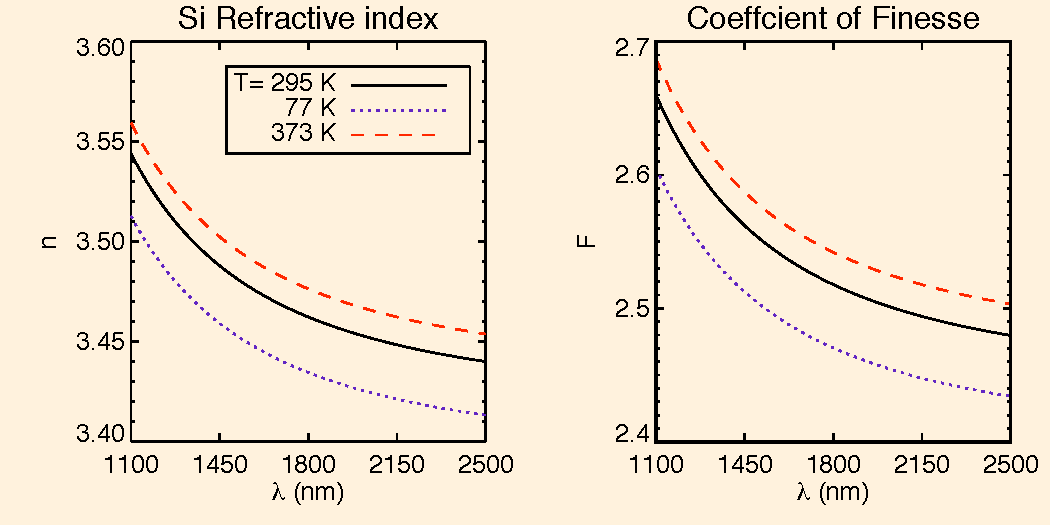
\includegraphics[width=0.95\columnwidth]{figs/SiIndexAOmgsFinesseFig.pdf}}
\caption{Plot of refractive index, $n$, and coefficient of finesse, $F$, as a function of wavelength, $\lambda$.\label{fig} We computed the temperature dependent refractive index from the tabulations of \cite{2006SPIE.6273E..77F}, and extrapolated past their upper temperature bound to estimate values near 373 K.  The coefficient of finesse is defined in Equation \ref{eq:FabPerot}.  The minuscule temperature dependence is largely negligible, and for the rest of the paper we assume room temperature refractive index.}
\end{figure}

The Si-air\footnote{We imprecisely refer to the gap as an air gap, though in principle the gap has an unknown mixture of gases for example water vapor, or other vapors that were outgassed from reactions catalyzed by hydrocarbons.} interfaces of the in the bond gap make a Fabry-P\`erot etalon\cite{2007fuph.book.....S}.  The transmission through a Fabry-Perot depends on the wavelength of light, the reflectivity of the etalon sidewalls, and the size of the gap.  We assume transmission is at normal incidence, the index of the gap is 1.0, and the material is at room temperature.  We assume Si is nonabsorbing longward of $\lambda$ = 1150 nm.  We compute the reflectivity for an Si-air interface, which is a modest function of wavelength through the refractive index of Silicon, $n(\lambda, T)$ \cite{2006SPIE.6273E..77F}.  The computation is simply Fresnel's law at normal incidence:

$$
R = \frac{(n-1)^2}{(n+1)^2}
$$

The reflectivity is about 30\% in the wavelength range 1100 to 5000 nm.  The modest wavelength dependence is shown in the bottom curve of the figure below.  The coefficient of Finesse\cite{2007fuph.book.....S} encapsulates the Fabry-P\`erot etalon's dependence on the reflectivity.  We compute a coefficient of Finesse in the range of about 2.7$-$2.9 depending on the wavelength.


\subsection{Consideration of multiple incoherent reflections}
\label{secTheory}
Multiple incoherent reflections occur within the Si substrate.  Treatment for multiple coherent reflections have been described in detail in the optics literature \cite{2007fuph.book.....S}.  The wave transfer matrix technique treats each dielectric interface as a matrix with elements relating the pre- and post- interface complex amplitudes in the left and right directions.  I adapted the wave transfer technique for incoherent interactions \cite{2002ApOpt..41.3978K}.  Specifically I constructed an incoherent wave transfer matrix whose elements relate the intensities (and not complex amplitudes) before and after an interface.  The details are worked out in Appendix \ref{sec:Append-IMRTMM}.  We computed the transmission for two scenarios- first a double side polished (DSP) Si puck with no air gap, and second a pair of bonded Si pucks with a gap thickness $d$.  The DSP Si puck with no air gap has a transmission equal to:

$$
T_{DSP} = \frac{2n}{1+n^2}
$$

which has an average value of about 53\%, as shown in the top curve of the Figure above.  Note that this transmission is above a na\"ive value of $T_{DSP}=(1-R^2)$, which does not take into account multiple incoherent reflections, and is therefore an underestimate.  If the Si wafer path length is less than the coherence length for the given spectral bandwidth, then the multiple reflections would interfere coherently, and the Si wafer would behave as a Fabry-P\`erot etalon.  We work out this behavior in the Appendix section X and show that in the limit $l>> \lambda^2 / \delta \lambda $ the spectral transmission tends to equation X.  

For the case of a pair of bonded Si pucks with a gap thickness $d$, we normalize the transmission with a gap to the transmission with no gap to isolate the effect of the gap.  We call this normalized transmission the etalon transmission $T_{e}$.  It is derived in Equation \ref{eqn:Tetalon} in the Appendix:


$$T_{e} = \frac{n^2+1}{2 n F \sin ^2(2\pi \frac{d}{\lambda})+n^2+1} \label{eqFP}$$


It is clear that in the limit $\lim_{d \rightarrow 0}$, the etalon approaches 100\% transmission.  In the next section we compare measurements to by-eye fits of this equation.


\section{Substrate preparation}
It is important to clean the wafers to minimize the particle density, since particles cause gaps.  The substrates were silicon wafers.  The surface roughness was typically about 2 nm, as measured with a Veeco NT9100 Optical Profiler .  The substrate thicknesses ranged from 0.5 to 3.3 mm per substrate.  We classify the 3.3 mm thick substrates as ``pucks'' and the $\sim$1.0 mm thick substrates as ``wafers''.  The distinction between the two classes of substrate thickness is based on the anticipation that thin substrates will conform more easily to their bonding partner substrates.  There is also evidence that bond front propagation is much slower in thick pucks \cite{2007ApOpt..46.6793H} than in wafers.  We measured the large scale surface flatness of the pucks.  The Fisba2 interferometer has a 2 inch diameter beam at $\lambda=$632.8 nm.  We found a typical peak to valley surface flatness of 2 waves over the central 2 inch diameter.


The detailed bonding procedure will be chronicled in a future paper.  Briefly, we prepared the substrates with standard cleaning procedures.  We used MHz frequency oxygen plasma ashing.  We soaked the wafers in DI water then dried with an N$_2$ gun.  We pressed the wafers together from the center.


\section{Measurement strategy, conditions, and details}
The measurements were performed with an Agilent Cary 5000 UV-Vis-NIR spectrophotometer \nocite{cary5000web}.  The typical measurement parameters and tool performance are listed below.  More details about the tool are available at the vendor's website.  Briefly, the tool has a double monochromator.  The double monochromator feature reduces scattered light, with the vendor reported linearity exceeding 40 dB.


The Cary 5000 has four operation modes: single front, single back, double, and double reverse.  We experimented with single front and double modes.  Double mode takes a reference spectrum simultaneously to the target spectrum.  In both single and double beam mode a baseline scan is taken of air.  The baseline spectrum is the raw spectral response of the system, which is automatically divided out of subsequent spectra.  In single beam mode the baseline measurements must be repeated about every half hour.  We estimated the uncertainty and measurement repeatability of single and double modes in the following way.  We computed the RMS error and measurement repeatability in a single measurement by computing the standard deviation of the beam with no sample in a series of spectra taken immediately after a 100\% baseline scan.  The predicted mean level should naturally be 100\%.  We found that the mean value in single mode drifted by about 0.2\%.  The standard deviation of the featureless spectrum was typically 0.02\%, with some portions of the spectrum demonstrating increased uncertainty, perhaps attributable to atmospheric absorption. In double beam mode the spectrograph performance was much better.  We put a double side polished Si wafer in the reference beam, and no sample in the target beam during the baseline scan.  In this way the transmission spectrum of a target Si wafer is automatically normalized.  The double beam mode effectively divides out variations in the mean transmission levels attributable to lamp drift at 0.2\% in single beam measurements.  The drift in mean transmission level is merely 0.02\% in double beam mode.  These values are accurate for measurements over a half hour timescale or less.  Over periods of hours the drift increases for both single and double beam mode, so a repeat baseline scan is sometimes necessary.  The need for repeat baselines is more acute for single mode.


The choice of spectral sampling was straightforward.  We expect smoothly varying spectral features for small ($<$ 1 $\mu$m) size gaps in Si bonded wafers.  Sampling theory dictates a few spectral resolution elements over the spectral feature of interest.  The Fabry-P\`erot fringes will be well-sampled so long as the gap is less than $\sim$100 $\mu$m.  Such large gaps would be easily detectable by other means.  So we simply pick the largest slit width, and therefore the lowest spectral resolution that the Cary 5000 permits: 5 nm.  We then sample the spectral resolution with $\sim$2.5 samples per spectral resolution element, 2.0 nm samples. 


Table \ref{tab:tablenum3} shows some properties of the Cary5000.


%\caption{Summary of Cary 5000 Measurement parameters \label{tab:tablenum3}}
\begin{center}
    \begin{tabular}{l l}
        Parameter (Units) & Value \\ 
        Spectral sampling interval (nm) & 2.0 \\
        Spectral resolution (nm) & 5 \\
        Time per sample (s) & 0.1 \\
        Available measurement range (nm) & 175-3300 \\
        Typical measurement range (nm) & 1000-2500 \\
	Single mode RMS  (percent) & 0.02 \\
	Double mode RMS  (percent) & 0.002 \\
	Single mode mean drift (percent) & 0.20 \\
	Double mode mean drift (percent) & 0.02 \\
	Mean 0\% baseline correction (percent) & 0.03 \\
 	Beam size (mm x mm) & 2 x 8 \\
	Wavelengths of instrumental artifacts (nm) & stuff \\
        num1 & 1200 \\
        num2 & 1350 \\
        num3 & 1360-1450\\
        num4 & 1850 \\
        num5 & 1800-1950 \\
        num6 & 2000 \\
        Vendor-reported linearity range (dB) & 40 \\
        Directly measured linearity range (dB) & 24 \\
      \end{tabular}
\end{center}


We also looked for the indication of large gaps detectable as ``IR bubbles'' \cite{1992JEMat..21..669M} with the coarse IR imaging technique.  The detector was an IR Vista $\alpha$NIR infrared focal plane array, with 312 $\times$ 252 pixels, with 30 $\mu$m square pixels.  We used a 50 mm F/2 lens, with a fiber optic white light illumination source.  We estimate that the lamp-detector combination was sensitive to wavelengths in the range 1.1-1.6 $\mu$m.  The field of view sub-sampled the 4 inch diameter wafers, so we dithered the sample.  No effort was made to flat field the detector, so copious detector non-uniformities and vignetting are present in our images.  It was easy to detect IR bubbles despite the artifacts since the bubbles translate with the wafer during dithering.  We detected IR bubbles in all 3 of the bonded Si pucks on which we recorded IR images.  The bubble areal density varied from about 4 per wafer (100 mm diameter) to over 20 per wafer.  Naturally, the sample of control solitary DSP (unbonded) wafers show no such IR bubbles, which are entirely attributable to the gaps between bonded substrtes as discussed in the literature (see Section \label{secHistory}).  Figure \ref{IRbubble} shows an example of one of the IR bubbles in which several bright and dark fringes are clearly discernible.  No attempt at quantitative measurement was made on the IR images due to anecdotal evidence that the detector is non-linear.  The morphology was clear regardless of the detector response.  

\begin{figure}[htbp]
\centerline{\includegraphics[width=.8\columnwidth]{figs/IR_bubble.pdf}}
\caption{Photo of part VG09 with transmission image of a bubble highlighted\label{IRbubble}.  The right side photo shows the 75 mm diameter wafer with blue Sharpie rectangles indicating the position of different spectral measurements (as detailed in the next section).  The yellow circle in the photo highlights the outline of the location of an IR bubble we detected.  The bubble shows a couple of fringes over the effective wavelength range 1.1-1.6 $\mu$m.  This fringe pattern is consistent with a gap comparable to this measurement wavelength.  The pointlike measurement artifacts, Sharpie marker, and vignetting are perceptible in the raw IR image.  Our interpretation of the IR bubbles is robust against these artifacts.  The area surrounding the IR bubble appears to be mostly devoid of large (wavelength-scale) gaps, since the transmission is fairly uniform, and consistent with the brightest fringe of the IR bubble.  }
\end{figure}


\section{Results of infrared spectroscopy of bonded Si pucks}
\label{secResults}
In this section we describe the spectroscopy of bonded Si pucks.  In some instances IR imaging was available and was leveraged to target IR bubbles.  In other cases the IR imaging was not available or simply ignored, and spectra were taken at random positions on the wafer surface.  

\subsection{Constructing the predicted transmission}
We constructed the predicted transmission in the following way.  If IR imaging was unavailable, our optimistic prior belief was simply that the bond should be perfect and indistinguishable from a solitary DSP Si wafer, (i.e. 100\% relative transmission).  For the cases where we had bored gaps of known dimension and fill factors we could predict the transmission with the Fabry-Perot machinery described in section ref{secTheory}, specifically equation \ref{eqFP}.  For non-unit fill factor, we simply average 100\% transmission with the predicted gap transmission, weighted by the estimated fill factor.  Notably the meshes we designed were all 50\% fill factor.  No attempt was made to verify the delivered fill factor, but since high precision lithographic processes were employed, we take the design fill factor as gospel.  The depth of the meshes has an associated uncertainty listed in \ref{tabbondexper}.  We incorporated the uncertainty in the mesh depth in the following way.  We computed the transmission curve for the 1$\sigma$ lower and upper bounds, and plot a filled band marked as the prediction band.  The uncertainties in the mesh depths were low enough that the band spread includes all intermediate lines of predicted transmission between plus and minus 1$\sigma$.  In cases where the IR imaging was unavailable the mesh position was only coarsely known, so our prediction band had to incorporate our uncertainty about whether or not our measurement beam was on or off or overlapping the mesh border.  If the beam was off the mesh we assumed 100\% relative transmission, so we simply set the lower bound of the predicted transmission to the equivalent of a zero gap.  

\subsection{Spectra of pucks with known gap sizes}
Figures \ref{VS21specm1} to \ref{VS21specf1} show examples of the predicted and measured IR spectra.  Figure \ref{VS21specm1} shows an example spectrum in which the measurement is consistent with the prediction for a gap with the known conditions.  Meanwhile, Figure \ref{VS21specf1} shows a spectrum in which the measurement marginally exceeds the prediction (by about $\sim 2 \sigma$).  Other parts show less consistency with the prediction.  A complete description of the diversity of the measured spectra requires an appeal to optical phenomena beyond the scope of this paper.  Briefly we classify the diversity of measurements into the categories laid out in the table below.  

\begin{figure}[htbp]
\centerline{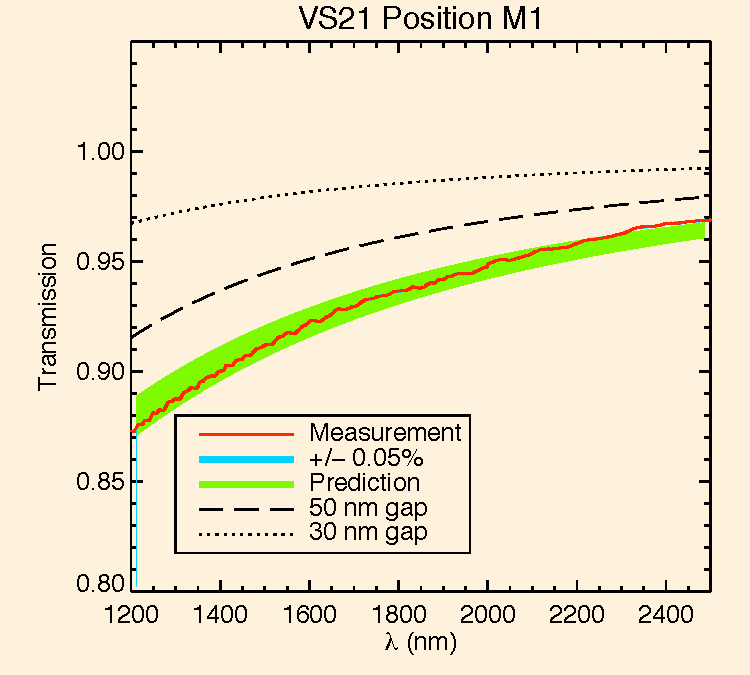
\includegraphics[width=.8\columnwidth]{figs/20130911_VS21posM1}}
\caption{IR transmission spectrum of VS21 (M1) showing consistent gap\label{VS21specm1}.  Example spectrum through part VS21 at a position through the mesh gap of known dimensions.}
\end{figure}

\begin{figure}[htbp]
\centerline{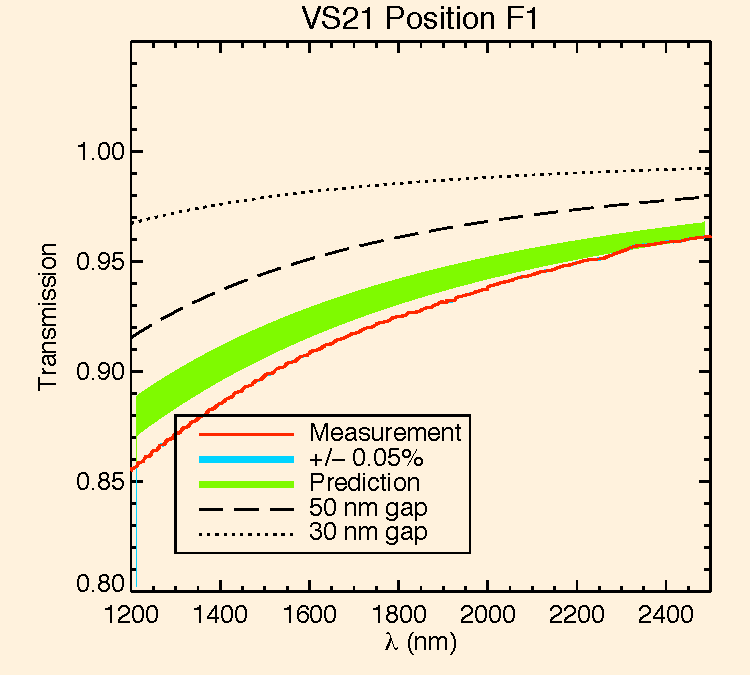
\includegraphics[width=.8\columnwidth]{figs/20130911_VS21posF1}}
\caption{IR transmission spectrum of part VS21 (F1) showing evidence for an excess gap\label{VS21specf1}.  Example spectrum through part VS21 at a position through the mesh gap of known dimensions.}
\end{figure}


\begin{table}[h!]
  \caption{Interpretation of the diversity of IR spectra}
  \begin{center}
    \begin{tabular}{ |p{8cm}| p{8cm} | p{2.2cm} |}
    \hline
    Appearance of spectra & Interpretation & Exemplars \\
    \hline
    Measurement within the prediction band & Life is good & VS21-M1, Figure \ref{VS21specm1}, VG15, VG07\\
    \hline
    Measured spectrum below the prediction band but shape is similar & Gap was slightly larger than predicted or bonding was incomplete& VS21-F1, Figure \ref{VS21specf1}, VS09, VG15, \\
    \hline
    Measured spectrum above the prediction band but shape is similar & Gap was slightly smaller than predicted & VS21-M2\\
    \hline
    Measured spectrum exceeds DSP reference puck & unanticipated anti-reflection coating on the surface of the Si sample (e.g. Sharpie marker residue) & VG08\\
    \hline
    High frequency, low amplitude wiggles superimposed upon smooth underlying trend & Large, unanticipated gap, with a small fill factor  & VS21-C3\\   
     																			     & wavelength dependent diffraction from the mesh patterns & VS21-C3\\       
     																			     & measurement artifact  & VS21-C3\\       												
    \hline
    Non-unit transmission constant with wavelength (gray spectrum) & Artifact of measurement- vignetting of beam, absorptive coating, zero-point drift & VS21-C4 \\
    \hline
    Completely different spectrum than anticipated with low absolute transmission & Large, inhomogeneous gap consistent with an IR bubble & VG09 \\
    \hline
    \end{tabular}
  \end{center}
\end{table}

A key result of this work is to show that gaps of known dimensions are recovered in our spectroscopy.  The cases in which predicted spectroscopy differs from measurement are due to either a bona-fide detection of a gap above and beyond the implanted gap, or some measurement artifacts.  In the next section we address mitigation of artifacts.

\subsection{Mitigation of measurement artifacts}
The principle artifacts and their interpretation are listed in table \ref{1}.  We mitigated the artifacts in the following ways.  For the Sharpie marker behaving as an anti-reflection (AR) coating, we simply removed the sharpie with IPA.  We have mostly been able to rule out wavelength-dependent diffraction from the mesh pattern as a measurement artifact, since the beam size is large and the angular spread of diffraction from the mesh pattern would be much smaller than the spread of the beam.  Still, to remove this concern, we moved to using the coarse mesh rather than the medium or fine meshes, when possible.  We saw no difference in the bond quality surrounding the medium or fine meshes, which is consistent with results from the literature (see the work of Mitani and collaborators from the mid 1990s).  Namely, Mitani showed that the gas pressure of bonded wafers grew as the fill factor of voids decreased.  In other words, what matters is the fill factor of voids, not their relative sizes.  Since the fine, medium, and coarse meshes had the same fill factors, we anticipate no difference in the pressure of the voids, and therefore no difference in the bonding properties.

\subsection{Non-normal incidence angles}
For the vast majority of applications, normal incidence performance is the quantity of interest.  The technique laid out in this paper outlines an approach for measuring the gap size of bonded Si wafers at normal incidence.  In principle, from there the performance at non-normal incidence can be worked out either by simulation or calculation.  Here we briefly motivate the challenge of experiment and simulation at non-normal incidence.  

\begin{figure}[htbp]
\centerline{\includegraphics[width=0.95\columnwidth]{figs/Sibondedprismcartoon.pdf}}
\caption{Schematic of a bonded Si immersion grating\label{figSiPrism}.  }
\end{figure}

Our final application that motivated this project is to make diffraction gratings on the hypotenuse of a silicon prism.  The diffraction occurs inside the silicon material and is dispersed and reflected back along its path.  This configuration is called an immersion grating.  Figure \ref{figSiPrism} shows a schematic of the geometry of our bonded Si immersion grating.  Our group has made monolithic immersion gratings for over a decade, but challenges in processing large (30 mm thick) Si wafers motivated an approach of patterning and processing thin (1-10 mm thick) Si wafers, and then bonding them to shaped and polished prisms.  This technique has been pioneered at SRON \cite{2012SPIE.8450E..2TV}.  In Figure \ref{figSiPrism} we show an example with a 10 mm thick Si puck bonded to a 25 mm thick, precision cut, shaped, and polished Si prism.  The group at SRON has patterned Si immersion echelle gratings on commercial thin  ($< 1$ mm) Si wafers.  Thin wafers have the drawback that they are conformal, so total-thickness-variations (TTV) directly translate into surface optical aberrations\cite{2012SPIE.8450E..2TV}.  

The consequence of our immersion grating design is a non-normal incidence interface in double pass.  In this case, the Fabry-P\'{e}rot framework developed here fails to predict the spectrum of the interface loss attributable to a finite albeit small (few nm) gap.  Specifically, complete internal reflection and evanescent waves will matter at large incidence angles, and the incoherent matrix technique is no longer accurate.  Polarization effects are important.  We do not have a mechanism for evaluating the bond performance until the final device is completed and its wavelength-dependent transmission is measured.  We can detect the performance degradation on final devices in the following nuanced way.  We will measure the efficiency of the bonded Si immersion grating as a function of both wavelength and angle.  Our group built a custom tool to make these measurements- the Custom Robotic Order, Wavelength, and Blaze Angle Recorder (CROWBAR) \cite{2012SPIE.8450E..2SG}.  Figure 3 in \cite{2012SPIE.8450E..2SG} shows the directly measured spectrum of a monolithic immersion grating.  Notably, the spectrum in Figure 3 in \cite{2012SPIE.8450E..2SG}  shows dozens of blaze peaks where the efficiency should be maximized.  A perfectly contacted Si$-$Si direct bonded optic would have identical performance to a monolithic counterpart.  Bonded immersion gratings with finite gap sizes will superimpose a wavelength dependent transmission loss on top of the blaze peaks.  In this way, the presence or absence of deleterious gaps can be identified in final immersion gratings.  One drawback of this approach is that gaps can only be identified after the costly process of producing the final optical device.  Large gaps identified this late in the game could render the costly optic useless, both in terms of efficiency and wavefront performance.  Our group is exploring the effectiveness of high-temperature annealing to eliminate IR bubbles in completed devices.


\subsection{Spectra of pucks with no implanted gap}
We have shown that the IR spectroscopy technique combined with the Fabry-P\'{e}rot framework provide accurate knowledge of the gap size.  In the cases where we expected no gap (i.e. perfect Si-Si bond), we have seen spectra consistent with 100\% transmission relative to a DSP Si wafer.  In other cases we have seen evidence for gaps, which is simply an indication that the bonding process introduces gaps.  In a followup paper we will describe ways to mitigate bond formation in bonded Si pucks.

\section{Conclusions}
We have shown a method for indirectly measuring the size of voids in bonded Si wafers.  The technique broadly applies to any compound Si optics measured at normal incidence.  We showed lab IR spectra with consistent predictions, and addressed ways to mitigate measurement artifacts. 

\appendix

\section{Appendix: X-ray Computed Tomography}
We acquired x-ray computed tomography of sample VG03.  The measurement details are listed in Table\ref{tab:tablenum4}.


%\caption{Summary of X-ray CT measurements for VG03 \label{tab:tablenum4}}
\begin{center}
    \begin{tabular}{ll}
    \emph{Parameter (Units)} & \emph{Value} \\ 
    Instrument& Xradia MicroCT \\
     Objective & 0.7X \\
    Accelerating voltage (kV) & 100 \\
        Power (W) & 10 \\
        Acquisition time (s) & 3.5 \\
        Number of views & 2521 \\
        Total slices & 469 \\
        Field of view diameter (pixels) & 988 \\
        Voxel lateral pixel resolution ($\mu$m) & 38.02 \\
        Estimate field of view (mm) & 37.5 \\
        Voxel axial pixel resolution ($\mu$m) & 0.5 \\
        Scan date & 2013 August 8 \\
        Sample thickness (mm) & 6.6 \\
     \end{tabular}
\end{center}

The axial resolution of the X-ray CT system is about 500 nm, which is much larger than the small ($\sim$ 15$-$90 nm) patterned gaps on many of our bonded samples.  Part VG03 has a cylindrical patterned gap with a $\sim$20 mm diameter and 4000 nm height.  We expected to see the cylindrical gap in about 8 resolution elements, given that the pattern was centered in the 25 mm diameter field of view.  We saw a circular feature that extended over 297 pixels, which corresponds to 11.3 mm, assuming the voxel lateral dimension from the table above, which is reported in the X-ray CT lab measurement details.  The feature...


\section{Incoherent Multiple Reflections Transfer Matrix Method}
\label{sec:Append-IMRTMM}

The wave transfer matrix method is described in detail in chapter 7 by Saleh and Teich in ``Fundamentals of Photonics'' \cite{2007fuph.book.....S}.  Briefly, their technique is to assemble a 2$\times$2 scattering matrix $\boldsymbol{S}$ which has the elements:
\begin{eqnarray}
\boldsymbol{S} = \left(
\begin{array}{cc}
 t_{12} & r_{21} \\
 r_{12} & t_{21} \\
\end{array}
\right)
\end{eqnarray}
Where $t$ and $r$ stand for transmission and reflection respectively.  The order of subscripts is the order of origin and destination of the wave in regards to the interface, so we know something about the direction of the wave and how it got there.  The $\boldsymbol{S}$ matrix encapsulates all the information we need to know about how light waves interact with the interface.  The real power of the matrix technique comes from a cousin of the scattering matrix, the so-called wave transfer matrix, $\boldsymbol{M}$.  The matrix $\boldsymbol{M}$ has the convenient property that its output can be used as the input for another matrix.  In other words, the input vector to $\boldsymbol{M}$ is made of the left and right moving components directly before the interface; the outputs are the left and right moving components directly after the interface:
\begin{eqnarray}
\left(
\begin{array}{c}
 U_2^{(+)} \\
 U_1^{(-)} \\
\end{array}
\right)=\boldsymbol{S} \left(
\begin{array}{c}
 U_1^{(+)} \\
 U_2^{(-)} \\
\end{array}
\right) \\
\left(
\begin{array}{c}
 U_2^{(+)} \\
 U_2^{(-)} \\
\end{array}
\right)=\boldsymbol{M} \left(
\begin{array}{c}
 U_1^{(+)} \\
 U_1^{(-)} \\
\end{array}
\right)
\end{eqnarray}

The elements of $\boldsymbol{S}$ and $\boldsymbol{M}$ are related to each other by geometric transformations\cite{2007fuph.book.....S}.  Much of the literature on the transfer matrix method deals with applications related to thin films, in which the wavelength is comparable to the size of the dielectric layer.  For thin films the vector components $U_{i}$ represent the complex amplitudes of the electromagnetic waves.  The polarization state can be encapsulated in scattering matrix components\cite{2007fuph.book.....S}.  The intensities of the emergent spectrum can be computed from the absolute square of the complex amplitudes.  For thick films, the vector components are the intensities of the emergent spectrum, since waves are incoherent.  \cite{2002ApOpt..41.3978K} work out the general transfer-matrix method for optical multilayer systems with incoherent interference.  The key idea for the incoherent transfer matrix method approach is to populate a scattering matrix with elements equal to the (wavelength dependent) transmitted $T_i$ and reflected $R_i$ intensities of an interface or set of interfaces that act together.  Then, use the geometric transformations to construct the $\boldsymbol{M}$ matrix.  

The matrix for the Fabry-P\`erot etalon is calculated in the following way.  The first key idea is that I had to treat the entire air gap as an abstraction, a Fabry-P\`erot etalon.  We don't need to bother to consider the microscopic coherent interactions with the etalon transmission, all of that information is encapsulated in these equations for a Fabry-P\`erot etalon.

\begin{eqnarray}
 \delta = \frac{2\pi}{\lambda}2d \\
  F \equiv \frac{4R}{(1-R)^2} \\
 T_e = \frac{1}{1+F\sin^2(\delta/2)}  \label{eq:FabPerot}
\end{eqnarray}

with $\lambda$ the vacuum wavelength, $R$ the Fresnel reflection of silicon, and $F$ the coefficient of finesse.  The coefficient of finesse $F$ and the phase $\delta$ are the two parameters of the Fabry-P\`erot etalon.  The coefficient of Finesse encapsulates the Fresnel reflection and depends only on the Si refractive index which has a minute wavelength (and temperature) dependence.  The phase depends on the wavelength $\lambda$ and $d$ the air gap spacing: $\delta=\frac{2\pi}{\lambda}2d$ .  We assume the etalon is lossless, i.e. the etalon has no absorption $T_e+R_e=1$.  So the incoherent scattering and transfer matrices for the etalon are:

\begin{eqnarray}
\boldsymbol{S_e}&=&\frac{1}{1+F\sin^2{\delta/2}} \left(
\begin{array}{cc}
1 & F \sin ^2(\delta/2) \\
F \sin ^2(\delta/2) & 1 \\
\end{array}
\right) \nonumber \\
\nonumber \\
\boldsymbol{M_e}&=&\left(
\begin{array}{cc}
 1-F \sin ^2(\delta/2) & F \sin ^2(\delta/2) \\
 -F \sin ^2(\delta/2) & 1+F \sin ^2(\delta/2) \\
\end{array}
\right)
\label{eqn:EtalonMatrix}
\end{eqnarray}

I assembled the matrix for the Air-Si Fresnel interface in the following way.  First it is important to note that the matrix is the same whether the transmission is from Si to air or air to Si.  This reciprocity is not necessarily true for the complex amplitudes matrix, but our approach employs intensities not complex amplitudes.  The Fresnel interface is lossless.  The transmission and reflection are given by the Fresnel equation for normal incidence:
\begin{eqnarray}
T_n&=&\frac{4n_{Si}}{(n_{Si}+1)^2} \\
R_n&=&\frac{(n_{Si}-1)^2}{(n_{Si}+1)^2} \label{eq:FresnelTrans}
\end{eqnarray}
For clarity I will drop the subscripts from $n_{Si}$, since we have already set $n_{air}=1$ and there are no other dielectric interfaces to think about.  So the scattering and transfer matrices for the air-Si Fresnel boundary are:

\begin{eqnarray}
\boldsymbol{S_n}&=&\frac{1}{(n+1)^2} \left(
\begin{array}{cc}
4n & (n-1)^2 \\
(n-1)^2 & 4n \\
\end{array}
\right)  \nonumber \\
\nonumber \\
\boldsymbol{M_n}&=&\frac{1}{4n}\left(
\begin{array}{cc}
 -n^2+6  n-1 & ( n-1)^2 \\
 -( n-1)^2 & ( n+1)^2 \\
\end{array}
\right)
\label{eqn:SiAirMatrix}
\end{eqnarray}

Finally, we cascade the matrices together to compute the net transmission through the stack of abstractions.  The result is a $2\times2$ transfer matrix: $$\boldsymbol{M_{net}}=\boldsymbol{M_n}\boldsymbol{M_e}\boldsymbol{M_n}$$  From the matrix transformation equations \cite{2007fuph.book.....S} we know $M_{22}=1/T$.  Taking the inverse of the bottom right element of $\boldsymbol{M_{net}}$, we get the transmission $T_{net}$ through the net optical device: 

\begin{eqnarray}
T_{net}=\frac{2 n}{1+ 2n F\sin ^2(\delta/2)+n^2} \label{eqn:FPmatTrans}
\end{eqnarray}

Compare equations \ref{eqn:FPmatTrans} and \ref{eq:FabPerot}.  The revised transmission has picked up a few factors of 2 and $n$.  While we are at it, let's compute the matrix for the scenario with no intermediate etalon: there are simply two Fresnel interfaces with which light interacts incoherently.  This scenario is the model for a single DSP reference puck. The revised matrix multiplication is simply $\boldsymbol{M_{DSP}}=\boldsymbol{M_n}\boldsymbol{M_n}$.  Taking the inverse of the $M_{22}$ element, we find: 
\begin{eqnarray}
T_{DSP}=\frac{2 n}{n^2+1}\label{eqn:EqofSummedSlab}
\end{eqnarray}
which is identical to the result obtained by directly summing the intensities from multiple reflections:
\begin{eqnarray}
T_{DSP}=T^2 \sum_{i=0}^{N}R^{2i} \label{eqn:multsum}
\end{eqnarray}

It is informative to isolate the effect of the gap by dividing the measured bonded wafer transmission by the transmission of a reference DSP Si part.  We call this normalized transmission the etalon transmission $T_{e}$:
\begin{eqnarray}
T_{e} = T_{net}/T_{DSP} \\
T_{e} = \frac{n^2+1}{2 n F \sin ^2(\delta/2)+n^2+1} \label{eqn:Tetalon}
\end{eqnarray}

\section{Appendix: High spectral resolution coherent interference of thin substrates}

Throughout this article we have assumed that $L >> \lambda^2 / \delta \lambda$, so that the interference of the substrate is safely incoherent.  Another way of stating this criterion is that the spectral bandwidth is large enough that high spectral frequency fringes average out in a composite spectrum of low spectral resolution.  If we relax this assumption so that the Si substrate thickness is comparable to or smaller than the coherence length, we would begin to observe high frequency fringes in the transmission spectra.  In this appendix section we work out the transmission spectrum for two scenarios.  First, we work out the case of a DSP Si wafer of thickness $L$, with no gap.  Second we work out the case of two bonded Si wafers of thicknesses $L_1$ and $L_2$.  For both cases we consider infinite spectral resolution, then convolve the spectra with a finite spectral resolution to show that the spectrum tends to that derived using an incoherent assumption.  

\subsection{DSP Si wafer at high spectral resolution}
The Fabry-P\`erot etalon transmission is given in Equation \# X (currently, 5).  What we want to evaluate is:
  
$$
 <T_e> = \lim_{\sin^2(\delta/2) \to 0.5} \frac{1}{1+F\sin^2(\delta/2)} \\
 <T_e> = \frac{1}{1+F/2}
$$



\bibliographystyle{osajnl}
\bibliography{AO_bondedSi}


%\begin{thebibliography}{99}

%% Do not include separate BibTeX files; if BibTeX is used,
%% paste the output (contents of .bbl file) here.

%\end{thebibliography}

\end{document}
